% Figure from MATH 591 notes, section 72 (Lecture 27). ADDED (not from lecture).
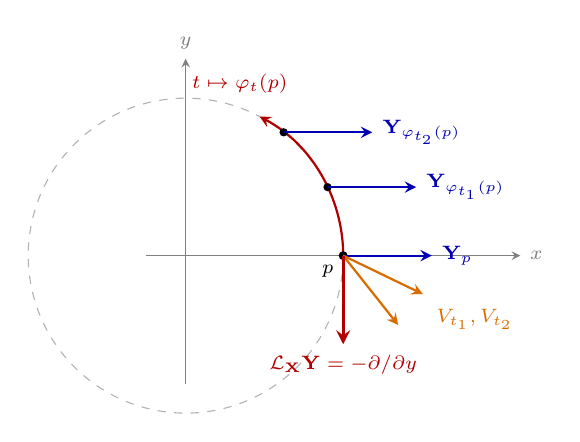
\begin{tikzpicture}[scale=1.25, >=stealth]
\draw[->, gray] (-0.4,0) -- (3.4,0) node[right, font=\scriptsize] {$x$}; \draw[->, gray] (0,-1.3) -- (0,2.0) node[above, font=\scriptsize] {$y$};
\draw[gray!60, dashed] (0,0) circle (1.6);
\draw[->, red!70!black, thick] (1.6,0) arc (0:62:1.6); \node[red!70!black, font=\scriptsize] at (0.55,1.75) {$t \mapsto \varphi_t(p)$};
\fill (1.441,0.696) circle (1.2pt); \draw[->, thick, blue!70!black] (1.441,0.696) -- ++(0.9,0) node[right, font=\scriptsize] {$\mathbf{Y}_{\varphi_{t_1}(p)}$};
\fill (0.995,1.253) circle (1.2pt); \draw[->, thick, blue!70!black] (0.995,1.253) -- ++(0.9,0) node[right, font=\scriptsize] {$\mathbf{Y}_{\varphi_{t_2}(p)}$};
\fill (1.6,0) circle (1.3pt) node[below left, font=\scriptsize] {$p$};
\draw[->, thick, blue!70!black] (1.6,0) -- ++(0.9,0) node[right, font=\scriptsize] {$\mathbf{Y}_p$};
\draw[->, orange!85!black, thick] (1.6,0) -- ++(0.810,-0.391);
\draw[->, orange!85!black, thick] (1.6,0) -- ++(0.559,-0.705);
\node[orange!85!black, font=\scriptsize, anchor=west] at (2.45,-0.65) {$V_{t_1}, V_{t_2}$};
\draw[->, very thick, red!70!black] (1.6,0) -- ++(0,-0.9) node[below, font=\scriptsize] {$\mathcal{L}_{\mathbf{X}}\mathbf{Y} = -\partial/\partial y$};
\end{tikzpicture}
